\section{EUTXO, Informally...}

\begin{frame}{UTXO vs EUTXO}

\centering

\tikzset{
  tx/.style =
  { draw = gray,
    shape = rectangle,
    align = center,
    minimum width=.5cm,
    minimum height=1.5cm },
  mid/.style =
  { draw,
    yshift=.5cm,
    shape = circle,
    inner sep = 0pt,
    minimum size=4pt },
  math/.style =
  { yshift=-.5cm },
  arg/.style =
  { anchor=center,
    align=left,
    font=\scriptsize },
  to/.style =
  { -,
    bend left = 30,
    thick },
  every matrix/.style =
  { column sep=2.2cm,
    ampersand replacement=\& },
  font=\small
}

\begin{tikzpicture}
  \matrix (mat) [matrix of nodes, nodes in empty cells] {
     \node[mid,red]   (a) {};
  \& \node[tx]        (b) {};
  \& \node[mid,red]   (c) {};
  \& \node[tx]        (d) {};
  \& \node[mid,black] (e) {};
  \\ \& \& \& \& \\
  };
  \path
  (a) edge[to, red]
  (b)
  (b) edge[to, black] node[arg, yshift=-.7cm] {x : Value\\ $\nu$ : Validator}
  (c)
  (c) edge[to, red] node[arg, yshift=.4cm] {$\rho$ : Redeemer}
  (d)
  (d) edge[to, black]
  (e)
  ;
  \node[math,fit=(mat-2-1)(mat-2-5)]{$\nu(\rho) \overset{\text{\tiny ?}}{=} \s{True}$};
\end{tikzpicture}
\vspace{.5cm}
\noindent\hfil\rule{0.9\textwidth}{.4pt}\hfil
\begin{tikzpicture}
  \matrix (mat) [matrix of nodes, nodes in empty cells] {
     \node[mid,red]   (a) {};
  \& \node[tx]        (b) {};
  \& \node[mid,red]   (c) {};
  \& \node[tx,label=below:\scriptsize$\sigma$ : State] (d) {};
  \& \node[mid,black] (e) {};
  \\ \& \& \& \& \\
  };
  \path
  (a) edge[to, red]
  (b)
  (b) edge[to, black] node[arg, yshift=-1cm] {x : Value\\ $\nu$ : Validator\\ $\delta$ : Data}
  (c)
  (c) edge[to, red] node[arg, yshift=.4cm] {$\rho$ : Redeemer}
  (d)
  (d) edge[to, black]
  (e)
  ;
  \node[math,fit=(mat-2-1)(mat-2-5)]{$\nu(\rho,\ \delta,\ \sigma,\ x) \overset{\text{\tiny ?}}{=} \s{True}$};
\end{tikzpicture}

\end{frame}

\begin{frame}{Contract Continuity}
\begin{itemize}
\item New data value on outputs
\item More information available to validators
\item We show that Cardano can model a specific form of state machine
  \begin{itemize}
  \item However, much more computational patterns are possible
  \item e.g. the entirety of \alert{Marlowe}, a DSL for financial contracts, has
been implemented as a state machine on top of EUTXO.
  \end{itemize}
\end{itemize}
\end{frame}

\begin{frame}{Example: Multi-signature Contract}

\begin{itemize}
\item \textbf{n-out-of-m} signature scheme
\item Plain UTXO requires off-chain communication
\item Can be expressed as a simple state machine:
\end{itemize}

\centering
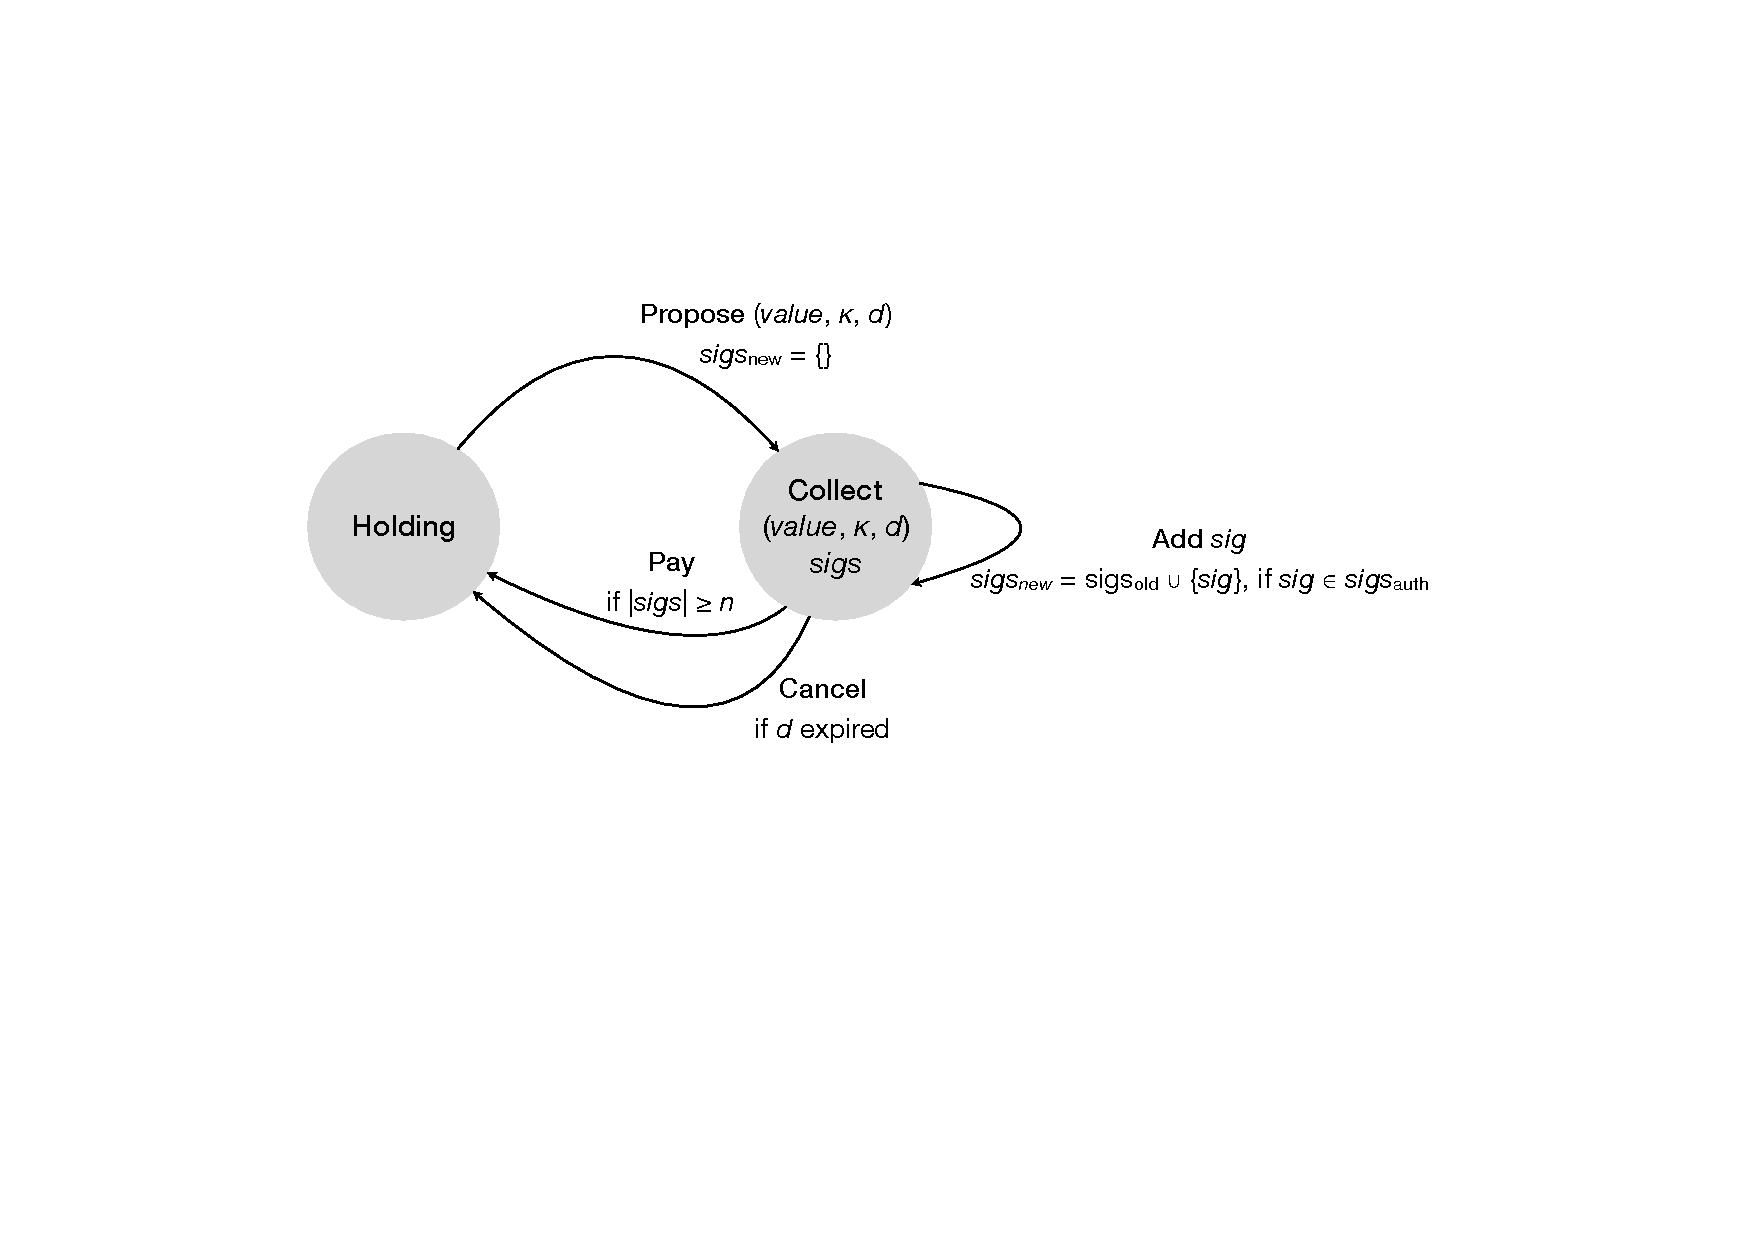
\includegraphics[width=\textwidth]{EUTxO_MultiSig_States.pdf}

\end{frame}

\begin{frame}{Example: Implementation in EUTXO}

\begin{itemize}
\item State machine is associated to a \textit{validator} function
\item \textit{Data values} in outputs correspond to states
  \begin{itemize}
  \item $\in \{ \msf{Holding} , \msf{Collecting} \}$
  \end{itemize}
\item Validator takes one of four possible transitions
  \begin{itemize}
  \item $\in \{ \msf{Propose} , \msf{Add} , \msf{Cancel} , \msf{Pay} \}$
  \item Choice provided by the \textit{redeemer} of the spending input
  \end{itemize}
\end{itemize}

\end{frame}
